\begin{figure}[!b]
    \centering
    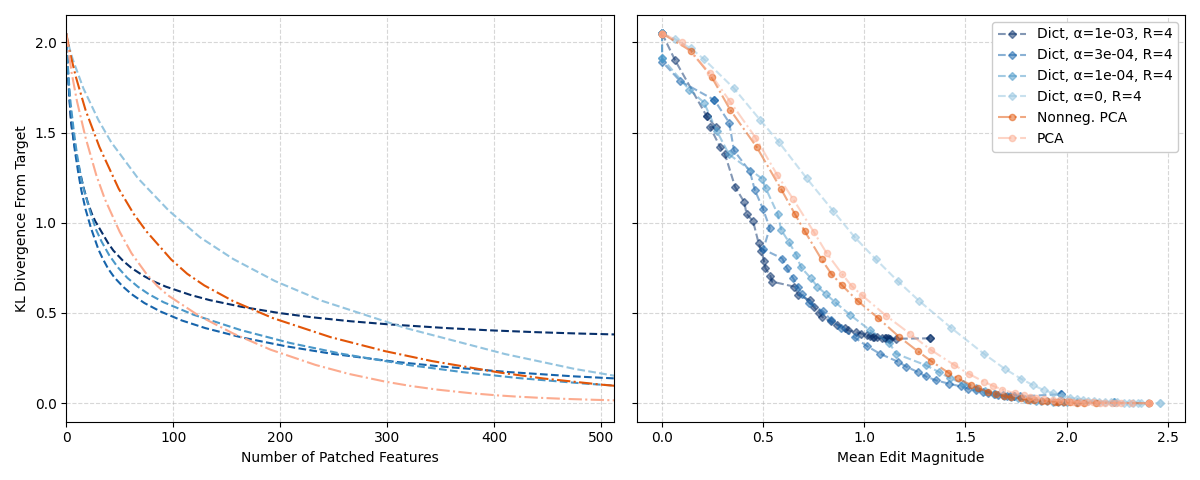
\includegraphics[width=\textwidth]{images/aidan/untitled/feature_ident_curve_l11.png}
    \caption{(Left) Number of features patched vs KL divergence from target, using various residual stream decompositions. We find that patching a relatively small number of dictionary features is more effective than patching PCA components and features from the non-sparse $\alpha=0$ dictionary. (Right) Mean edit magnitude vs KL divergence from target as we increase the number of patched features. We find that our sparse dictionaries improve the Pareto frontier of edit magnitude vs thoroughness of editing. In both figures, the feature dictionaries were trained on the first 10,000 elements of the Pile \citep{gao2020pile} (approximately 7 million activations) using the indicated $\alpha$ and $R$ values, on layer 11 of Pythia-410M (see Appendix \ref{appendix:ioi_other_layers} for results on other layers).}
    
    
    % \begin{minipage}[b]{0.49\textwidth}
    %     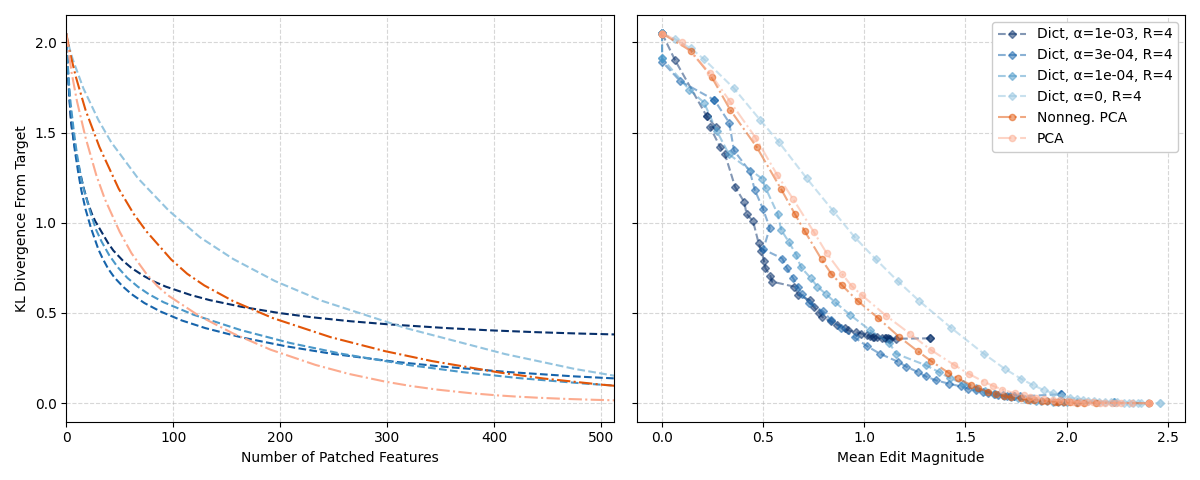
\includegraphics[width=\textwidth]{images/aidan/untitled/feature_ident_curve_l11.png}
    % \end{minipage}
    % \hfill  % Optional: To make sure they are as far apart as possible.
    % \begin{minipage}[b]{0.49\textwidth}
    %     \includegraphics[width=\textwidth]{images/aidan/untitled/feature_ident_curve_edit_l11.png}
    % \end{minipage}
    \label{fig:ioi-feature-identification}
\end{figure}

In this section, we quantify whether our learned dictionary features localise a specific model behaviour more tightly than the PCA decomposition of the model's activations. We do this via activation patching, a form of causal mediation analysis \citep{vig2020investigating}, through which we edit the model's internal activations along the directions indicated by our dictionary features and measure the changes to the model's outputs. We find that our dictionary features require fewer patches to reach a given level of KL divergence on the task studied than comparable decompositions (Figure \ref{fig:ioi-feature-identification}).

Specifically, we study model behaviour on the Indirect Object Identification (IOI) task \citep{wang2022interpretability}, in which the model completes sentences like ``Then, Alice and Bob went to the store. Alice gave a snack to \underline{\hspace{5mm}}''. This task was chosen because it captures a simple, previously-studied model behaviour. Recall that the training of our feature dictionaries does not emphasize any particular task.


\subsection{Adapting activation patching to dictionary features}
\label{subsec:activation patching}


In our experiment, we run the model on a counterfactual target sentence, which is a variant of the base IOI sentence with the indirect object changed (e.g., with ``Bob'' replaced by ``Vanessa''); save the encoded activations of our dictionary features; and use the saved activations to edit the model's residual stream when run on the base sentence.

In particular, we perform the following procedure. Fix a layer of the model to intervene on. Run the model on the target sentence, saving the model output logits $\mathbf{y}$ and the encoded features $\bar{\mathbf{c}}_1, ..., \bar{\mathbf{c}}_k$ of that layer at each of the $k$ tokens. Then, run the model on the base sentence up through the intervention layer, compute the encoded features $\mathbf{c}_1, ..., \mathbf{c}_k$  at each token, and at each position replace the residual stream vector $\mathbf{x}_i$ with the patched vector

\[ \mathbf{x}'_i = \mathbf{x}_i + \displaystyle \sum_{j \in F} (\bar{\mathbf{c}}_{i,j} -\mathbf{c}_{i,j})\mathbf{f}_j\]

where $F$ is the subset of the features which we intervene on (we describe the selection process for $F$ later in this section). Let $\mathbf{z}$ denote the output logits of the model when you finish applying it to the patched residual stream $\mathbf{x}'_1,...,\mathbf{x}'_k$. Finally, compute the KL divergence $D_{KL}(\mathbf{z}||\mathbf{y})$, which measures how close the patched model's predictions are to the target's. We compare these interventions to equivalent interventions using principal components found as in Section \ref{subsection:interpretability_baselines}.

To select the feature subset $F$, we use the Automated Circuit Discovery (ACDC) algorithm of \citet{conmy2023towards}. In particular, we use their Algorithm 4.1 on our features, treating them as a flat computational graph in which every feature contributes an independent change to the $D_{KL}$ output metric, as described above and averaged over a test set of 50 IOI data points. The result is an ordering on the features so that patching the next feature usually results in a smaller $D_{KL}$ loss than each previous feature. Then our feature subsets $F$ are the first $k$ features under this ordering. We applied ACDC separately on each decomposition.


\subsection{Precise Localisation of IOI Dictionary Features}

We show in Figure \ref{fig:ioi-feature-identification} that our sparse feature dictionaries allow the same amount of model editing, as measured by KL divergence from the target, in fewer patches (Left) and with smaller edit magnitude (Right) than the PCA decomposition. We also show that this does not happen if we train a non-sparse dictionary ($\alpha=0$). However, dictionaries with a larger sparsity coefficient $\alpha$ have lower overall reconstruction accuracy which appears in Figure \ref{fig:ioi-feature-identification} as a larger minimum KL divergence. In Figure \ref{fig:ioi-feature-identification} we consider interventions on layer 11 of the residual stream, and we plot interventions on other layers in Appendix \ref{appendix:ioi_other_layers}.

\iffalse

We have shown that our decomposition identifies directions that are relevant to behaviour on the IOI task and concentrates that relevance into a smaller number of dictionary features than comparable decompositions, and in Appendix \ref{appendix:steering_vs_edit_mag} we show that our edits are also more finegrained (in that they achieve the same level of steering at a lower edit magnitude) than patching with PCA, implying potential applications in future model steering efforts. 


\fi
